\section{Evaluation Webframework}
\label{sec:evaluationwebframework}
\subsection{Kriterienkatalog}
Die folgende Kriterien wurden zusammen mit dem Industriepartner definiert und festgelegt:
\begin{itemize}
\item Open Source Software, keine Lizenzgebühren
\item Beispiel- und Referenzprojekte vorhanden
\item Hohe Performance und stabile Verfügbarkeit auch bei hoher Auslastung
\item Skalierbar für mehrere Rennen und Etappen
\item Datenbankanbindung an \textit{\gls{mariadb}}
\item Weiterentwicklung durch cnlab AG muss möglich sein
\end{itemize}
Optionale, gewünschte Anforderungen:
\begin{itemize}
\item Vorkenntnisse in der betreffenden Programmiersprache
\item Gleiche Technologie für \textit{\gls{api}}, Webseite und Datenverarbeitung
\item Umfangreiche Dokumentation und Tutorials (Community\footnote{Die Community ist die Verbreitung einer Technologie sowie die Hilfsbereitschaft in Foren und Portalen. Dies ist äusserts schwierig zu beurteilen und kann sich auch schnell ändern.})
\end{itemize}
\subsection{Mögliche Lösungen}
\subsubsection{Django}
Django ist ein auf Python basiertes Webframework. Es wird eingesetzt bei berühmten Webseiten wie z.B. Pinterest, Instagram und The Washington Post.  Django beinhaltet einen OR Mapper, Templates zur Darstellung und einen URL Dispatcher als Controller.
\subsubsection{Spring MVC}
Spring MVC ist ein Framework für die Erstellung von Webprojekten. Es basiert auf Java Technologien und fördert Dependency Injection  und aspektorientierte Programmierung.
\subsubsection{JavaServer Faces}
JSF ist ein Framework-Standard für Webapplikationen in Java. Es verwendet die Java Servlet Technologie und benötigt einen Servlet Container für den Betrieb. Mit JSF können Komponenten für User Interfaces einfach in Webseiten eingebaut werden. 
\subsubsection{Symfony}
Symfony ist ein Open Source PHP Webframework und verfolgt das MVC Pattern. Die Zuordnung der Models geschieht dabei über die Namensgleichheit in Singular und Plural und nicht über Konfigurationsdateien (convention over configuration). Weiter können durch Konsolenapplikationen Anwendungen generiert werden.
\subsubsection{Ruby on Rails}
Rails ist ein Webframework geschrieben in Ruby. Es ist geprägt von den Prinzipien „don’t repeat yourself“ und „convention over configuration“. Ruby on Rails besteht aus fünf Modulen, jedes dieser Module übernimmt gewisse Funktionen, so z.B. der Action Mailer versendet und empfängt E-Mails.
\subsection{Nutzwertanalyse}
\begin{figure}[H]
	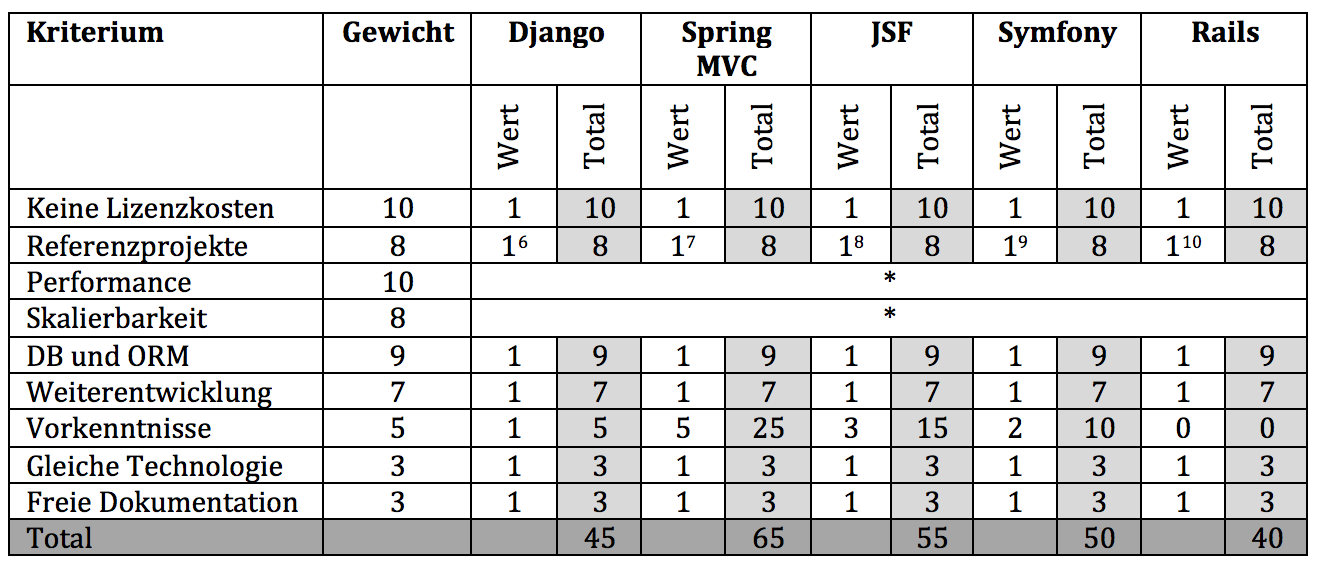
\includegraphics[width=130mm]{images/tourliveweb/nutzwertanalyse.png}
	\caption{Nutzwertanalyse}
\end{figure}
\subsubsection{Erläuterung zu Performance und Skalierbarkeit}
Bezüglich der Performance gibt es verschiedene Ansichten zu den verschiedenen Frameworks. Da es aber zu allen obigen Frameworks grosse Projekte gibt, kann davon ausgegangen werden, dass die Performance und Skalierbarkeit für das TourLive Projekt ausreicht.
\subsubsection{Erläuterung zur Gewichtung der Kriterien}
Die verschiedenen Kriterien wurden in einer Skala von 1 – 10 gewichtet, wobei 10 das wichtigste Kriterium darstellt. Gemäss cnlab Software AG dürfen für das Framework keine Lizenzkosten anfallen und die Webseite muss auch unter Last stabil verfügbar sein. Daher werden diese beiden Kriterien mit dem höchsten Gewicht 10 versehen.
Da das System einen stark wachsenden Datenbestand haben wird, ist die Implementation von Datenbanken ebenfalls von grosser Bedeutung. Referenzprojekte dienen als Beweis für die Skalierbarkeit und die Performance des jeweiligen Frameworks.
Für die Studierenden ist der Zugang zu freier Dokumentation sowie Vorkenntnisse relevant, jedoch nicht zwingend erforderlich. Wünschenswert ist ebenfalls, dass für das gesamte Webprojekt dasselbe Framework verwendet werden kann. Diese Punkte werden daher mit den Gewichten 3-5 bewertet.
\subsubsection{DB und ORM}
Ruby on Rails verfolgt das Ziel möglichst abstrakt mit Datenbanken zu arbeiten und kann deshalb problemlos mit verschiedenen Datenbanksystemen arbeiten. Gleiches gilt für den Ansatz bei Django, dort werden verschiedene Datenbankadapter zur Verfügung gestellt. Auch Spring arbeitet z.B. mit Hibernate als ORM problemlos mit verschiedenen Datenbanken.
\subsubsection{Weiterentwicklung durch cnlab Software AG}
Nach Abschluss der Arbeit wird das Projekt durch die cnlab weiterentwickelt. Daher muss bei der Auswahl des Frameworks darauf geachtet werden, dass eine weitere Entwicklung möglich ist.
\subsubsection{Schlussfolgerungen}
Da die Frameworks sehr ähnliche Ansätze verfolgen und aktuell eine grosse Entwicklergemeinschaft geniessen, sind die Unterschiede, abgesehen von der Programmiersprache welche als Grundlage dient, sehr klein. Entscheidend sind schliesslich die Vorkenntnisse: Java ist diejenige, für die bereits das grösste Vorwissen besteht. Daher sind für die engere Wahl die beiden Lösungen Spring MVC und JSF im Rennen. Da wir in einer kleinen Projektarbeit bereits mit JSF gearbeitet haben, möchten wir nach unseren eher negativen Erfahrungen damit von einer Entwicklung mit JSF absehen und auf das Spring MVC Framework setzen.

\subsection{Anmerkung zum Framework}
Das Java Spring MVC Webframework baut auf dem Prinzip \textit{Dependency Injection} auf. Dependency Injection wird unter anderem mit dem Begriff Inversion of Control zusammengefasst und im folgenden Abschnitt erläutert. Weiter fördert Spring gute Programmierpraktiken wie z.B. die Trennung von Model, View und Controller oder die Verwendung von Objekt relationalen Mappern beim Einsatz von Datenbanken in der Persitenzschicht.

\subsubsection{Dependency Injection}
Die Grundlage für Dependency Injection basiert auf dem Prinzip, dass möglichst wenig Abhängigkeiten eines Objekts von einem anderen Objekt besitzt werden. Die Abhängigkeiten sollen zur Verfügung gestellt werden. So kann unabhängig von der Implementation auf die Schnittstellen zugegriffen werden. Dies erlaubt zum Beispiel einen späteren Austausch der Abhängigkeit. In Spring übernimmt der Dependency Injection Container diese Aufgabe. Die benötigten Abhängigkeiten können entweder mit einer Annotation im Code oder durch Konfiguration in einer xml Datei deklariert werden. Die nachfolgende Grafik stammt von Martin Fowlers Artiekel zum Thema Dependency Injection \cite{martinfowler2004}.
\begin{figure}[H]
	\centering
	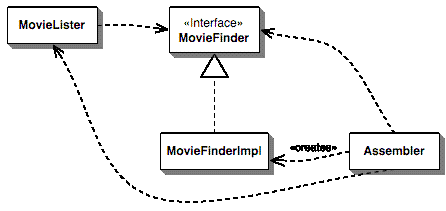
\includegraphics[width=100mm]{images/tourliveweb/dependencyinjection.png}
	\caption{Dependency Injection nach Martin Fowler \cite{martinfowler2004}}
	\label{fig:dpendencyinjection}
\end{figure}
Die Funktionsweise kann am einfachsten anhand des Beispiels von Martin Fowler in Abbildung \ref{fig:dpendencyinjection} aufgezeigt werden. Die Klasse MovieLister zeigt und filtert Filme. Dabei spielt die Quelle woher die Filme kommen keine Rolle. MovieLister benötigt nur eine Liste von Filmen (Abhängigkeit). Die MovieFinderImpl Klasse bietet genau diese Möglichkeit und zeigt dies durch die Implementation des MovieFinder Interfaces an. Der Assembler fügt die Abhängigkeit in den MovieLister ein (Injection).
\\

In dieser Weise können die Filme in einer Excel Datei, in einer Datenbank oder in einer Textdatei gespeichert werden, die Klasse MovieLister kann in jedem Fall verwendet werden.

\subsection{Spring Framework}
Für die Entwicklung von Webapplikationen bietet Spring das integrierte Modul \textit{MVC} an. Damit werden die grundlegenden Funktionalitäten einer Webapplikationen bereits abgedeckt.

\begin{figure}[H]
	\centering
	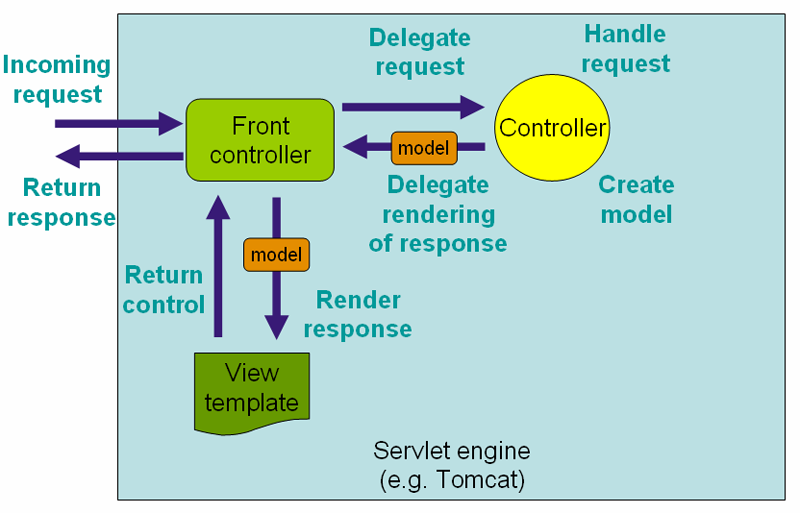
\includegraphics[width=130mm]{images/tourliveweb/springmvc.png}
	\caption{Aufbau von Spring MVC \cite{springsourcemvc2011}}
	\label{fig:springmvc}
\end{figure}

Die Anfragen werden durch den Front Controller empfangen und an den passenden Controller der Applikation weitergeleitet. Dieser fügt die angeforderten Daten (Model) hinzu. Das Model wird dann in die View Templates eingefügt und via den Front Controller an den Client zurückgeschickt.
\\

Dieses abstrakte Vorgehen kann durch ein konkretes Beispiel sehr gut dargestellt werden. Eine Anfrage wird durch den Aufruf einer URL im Browser ausgelöst (z.B. http://www.tourlive.ch/rennen). Der Front Controller sucht den Applikations Controller für die Ressource \textit{/rennen}. Bereitet das Model, in diesem Fall alle sichtbaren Rennen, vor und sendet dieses zurück. Der Front Controller sucht den View Resolver und übergibt das Model (alle sichtbaren Rennen). Dort wird das Model zur Darstellung gebracht und schlussendlich via den Front Controller an den Browser zurückgesendet. Für jede Ressource gibt es also einen Controller, dabei können aber auch generische Elemente wie z.B. der Rennname in der Ressource verwendet werden (z.B. http://www.tourlive.ch/rennen/tourdesuisse).
\\

Für die Einarbeitung in das Spring Framework wurden verschiedene Quellen verwendet. Alle Angaben dazu befinden sich im Literaturverzeichnis. Der obige Abschnitt ist eine Zusammenfassung von Inhalte aus den SpingSource Tutorials \cite{springsourcemvc2011} und Mkyong \cite{springmvcexamples2011} .